\include{template}
%\cfoot{} %% if no page number is needed

%\renewcommand\arraystretch{1.2}

\begin{document}

\begin{header}
TP

Dissolution -- Sauvez Maurice !
\end{header}

\section*{Contrainte}

Chaque élève rédige un compte-rendu qui fera partie du cours.

\section*{Prélude}

\begin{doc}
\textbf{1 : Concentration massique}

La concentration massique d'une solution exprimée en g/L, aussi appelée titre massique, indique la masse (en gramme) de soluté dissous dans un litre de solution.
Elle est donnée par :
\begin{equation}
C_m = \frac{m_\mathrm{soluté}}{V_\mathrm{solution}}.
\nonumber
\end{equation}
\end{doc}

\begin{enumerate}
\item \rea{} Déterminer la masse de sel à prélever pour préparer 50\,mL de solution d'eau salée de concentration 84\,g/L.
\item \anarai{} Proposer un protocole pour préparer cette solution.
\item \anarai{} Établir la liste du matériel nécessaire.
Si vous voulez utiliser du matériel qui n'est pas dans votre bac, vous pouvez demander à l'enseignant qui vous le prêtera si nécessaire.
\item \rea{} Réaliser la solution.
%\item \anarai{} \app{} Proposer un protocole pour mesurer la masse volumique de la solution obtenue.
\end{enumerate}

\section*{Quelle verrerie choisir ?}

\begin{center}
\begin{tabular}{ccccc}
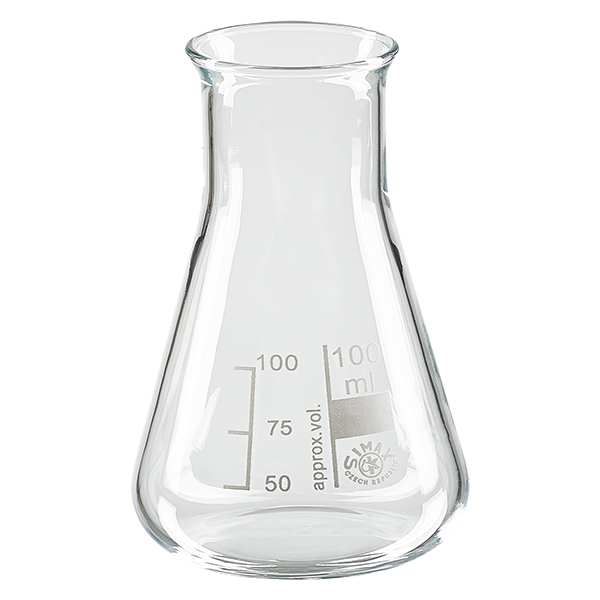
\includegraphics[height=90pt]{images/verrerie_erlenmeyer.jpg} &
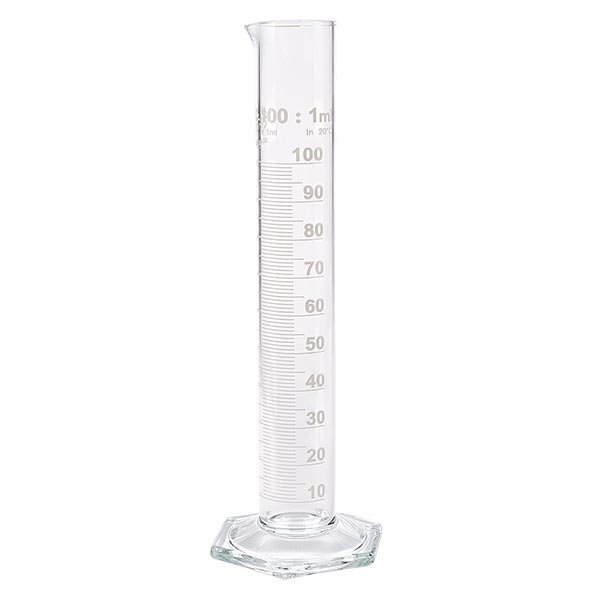
\includegraphics[height=90pt]{images/verrerie_eprouvette_graduee.jpg} &
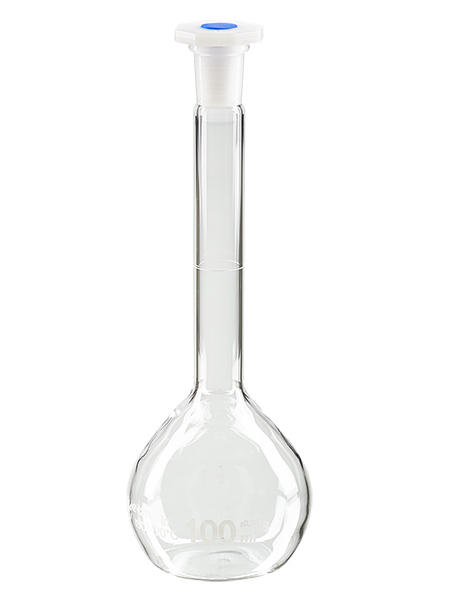
\includegraphics[height=90pt]{images/verrerie_fiole_jaugee.jpg} &
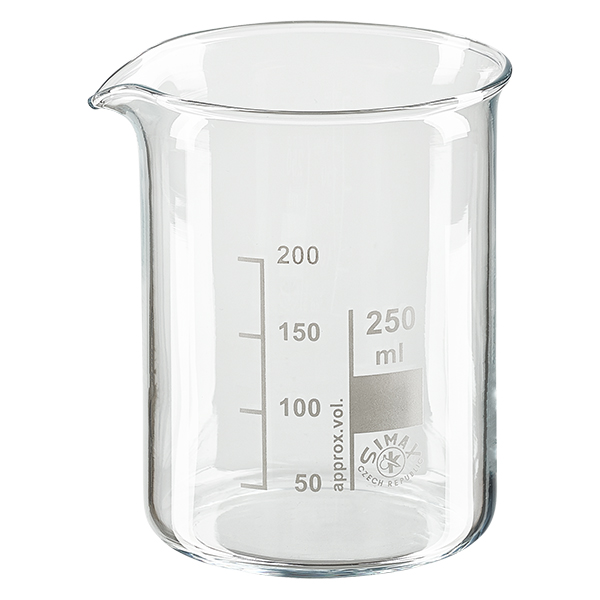
\includegraphics[height=90pt]{images/verrerie_becher.jpg} &
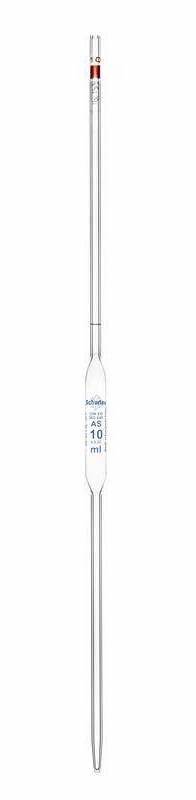
\includegraphics[height=90pt]{images/verrerie_pipette_jaugee.jpg} \\

\textbullet & \textbullet & \textbullet & \textbullet & \textbullet
\end{tabular}

\vfill

\begin{tabular}{l|c|c|c|c|c}
 & \textbullet & \textbullet & \textbullet & \textbullet & \textbullet \\
\textbf{Nom} & Becher & Erlenmeyer & Eprouvette graduée & Fiole jaugée & Pipette jaugée \\
\hline
\textbf{Contenance} & & & & & \\
\textbf{(mL)} & & & & & \\
\hline
\textbf{Incertitude} & & & & & \\
\textbf{(mL)} & & & & & \\
\hline
\textbf{Incertitude} & & & & & \\
\textbf{relative (\%)} & & & & & 
\end{tabular}
\end{center}

\section*{Sauvez Maurice !}

Comme d'habitude, Maurice pousse le bouchon un peu trop loin et dépasse les bornes des limites.
Grand oncle du célèbre Nemo, il cherche à s'évader de son bocal avec l'aide de son ami Florian le pélican.
Une maladresse de son dentiste de maitre a créé une fissure dans l'aquarium et de l'eau s'est échappée.
Le bocal a été réparé mais il est désormais à moitié vide ce qui rend l'attente du jour J très difficile.
Faute de pouvoir l'assister dans son entreprise d'évasion, vous devrez aider Maurice en remplissant son bocal.
Attention, Maurice est un poisson clown octogénaire sensible !
Vous ne pourrez pas lui donner n'importe quelle eau : il faut qu'elle respecte la salinité de son habitat naturel, les récifs tropicaux de l'océan pacifique.

Votre objectif :
\begin{objectif}
\textbf{Préparer 100\,mL d'océan pacifique}
\end{objectif}

\begin{doc}
\textbf{2 : Salinité de l'eau de mer}
\begin{multicols}{2}
\begin{center}
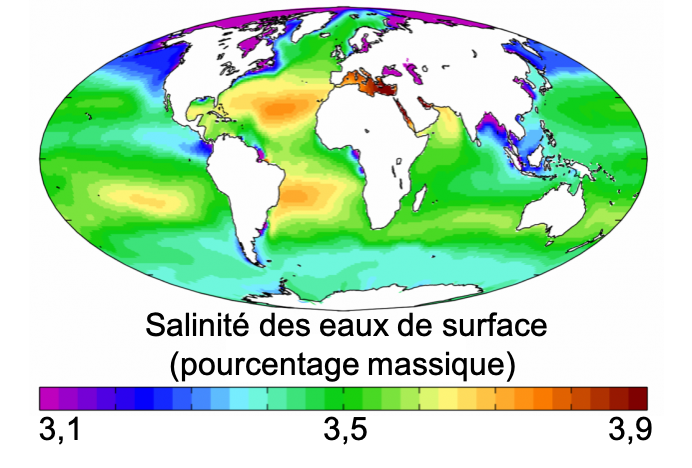
\includegraphics[scale=0.6]{images/salinite_fr.png}
\end{center}

L'eau de mer présente une grande concentration de sels dissous, majoritairement du chlorure de sodium  de formule chimique NaCl.
La salinité désigne la teneur en sel dissous.

La salinité de l'eau de mer varie à la surface du globe terrestre, en fonction de la latitude, de l'ouverture des mers vers les océans, de leurs dimensions, des apports terrestres, des courants...

\flushright \textit{Source : \href{http://doc.lerm.fr/salinite-leau-mer/}{doc.lerm.fr}}

\end{multicols}
\end{doc}

\begin{multicols}{2}
\begin{doc}
\textbf{3 : Salinité de quelques mers et océans}

\begin{center}
\begin{tabular}{l|c}
Mer considérée & Salinité en g/L \\
\hline
Mer Baltique   & 5{,}5 \\
Mer Noire       & 20{,}0 \\
Océan Pacifique & 35{,}0 \\
Mer Méditerranée & 40{,}0 \\
Mer Rouge & 54{,}0 \\
Mer Morte & 225 \\
\end{tabular}
\end{center}

\flushright \textit{Source : \href{http://doc.lerm.fr/salinite-leau-mer/}{doc.lerm.fr}}
\end{doc}
\end{multicols}

\end{document}